%------------------------------------------------
\begin{frame}
\frametitle{Compare and contrasts}
\hypertarget{compare}{}
\begin{columns}[c] % The "c" option specifies centered vertical alignment while the "t" option is used for top vertical alignment

\column{.5\textwidth} % Left column and width

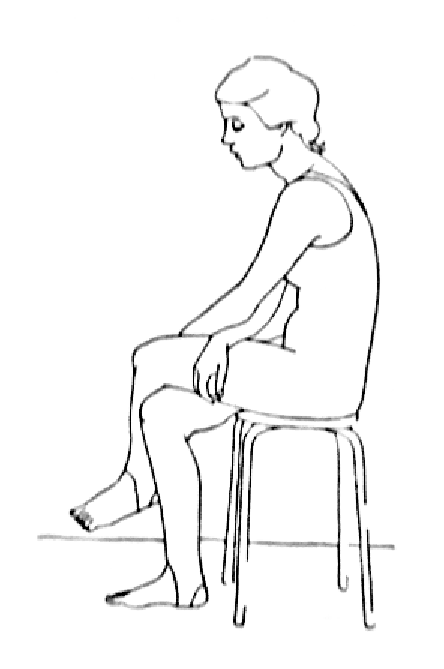
\includegraphics[width=0.7\linewidth]{Sitting_posture_Bad}

\column{.5\textwidth} % Left column and width
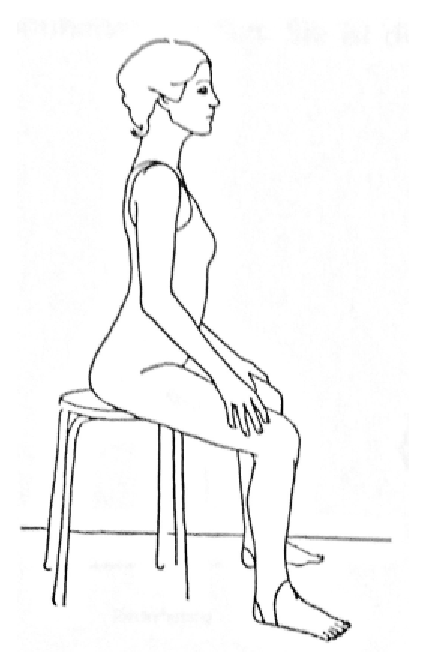
\includegraphics[width=0.75\linewidth]{Sitting_posture_Good}
\end{columns}
\end{frame}
%------------------------------------------------

\begin{frame}
\frametitle{Malposition}
\begin{columns}[c] % The "c" option specifies centered vertical alignment while the "t" option is used for top vertical alignment
\column{.4\textwidth} % Left column and width
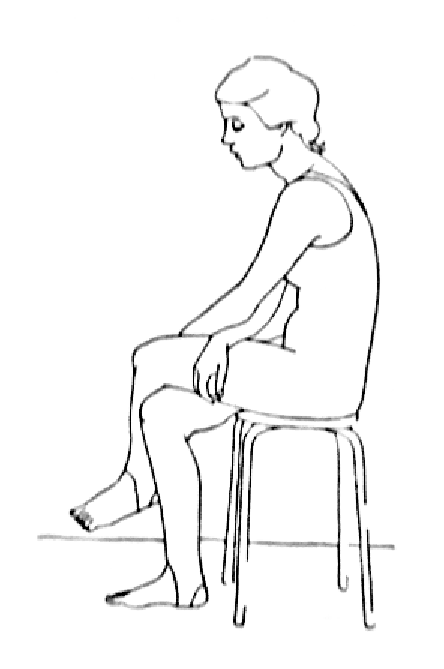
\includegraphics[width=1\linewidth]{Sitting_posture_Bad}
\column{0.7\textwidth} % Left column and width

\begin{itemize}
\item[1.] \structure{Sunken chest}
\item[2.] Hip erect
\item[3.] Kyphosis\footnote{Kyphosis: backwards curvature of the spine} with a big \structure{curvature} of the lumbar, thoracic and lower cervical \structure{spine}
\item[4.] Compensatory lordosis\footnote{Lordosis: forward curvature of the spine} of the central cervical spine
\item[5.] Reclination\footnote{Reclination: Backwards bending of the neck} of the upper cervical spine (``head joint'')
\item[6.] \structure{Forward falling of the shoulders}
\item[7.] Non--physiological leg and feet axes
\end{itemize}


\end{columns}
\end{frame}
%------------------------------------------------
%------------------------------------------------

\begin{frame}
\frametitle{Physiological Position}
\begin{columns}[c] % The "c" option specifies centered vertical alignment while the "t" option is used for top vertical alignment
\column{.4\textwidth} % Left column and width
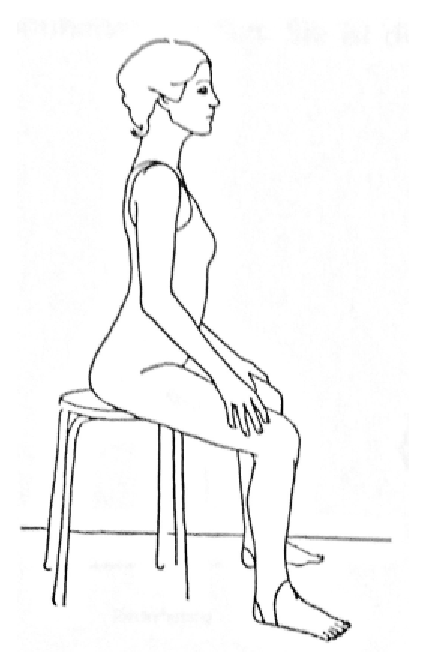
\includegraphics[width=1\linewidth]{Sitting_posture_Good}
\column{.7\textwidth} % Left column and width

\begin{itemize}
\item[1.] \structure{Chest lifted}
\item[2.] Hip tilted
\item[3.] harmonic thoracolumbal (chest--loin) \structure{lordosis} from the fifth thoracic vertebra to the sacrum.
\item[4.] Cervical spine (neck) stretched
\item[5.] Craniocervical inclination\footnote{Inclination: Forward bending of the head} (\structure{chin to larynx})
\item[6.] Retroposition\footnote{Retroposition: Backwards shift} of the shoulders (\structure{shoulder girdle rests on the thorax})
\item[7.] Physiological leg and feet axes
\end{itemize}


\end{columns}
\end{frame}
%------------------------------------------------
%------------------------------------------------

\begin{frame}
\frametitle{Habits influence our posture}
\begin{columns}[c] % The "c" option specifies centered vertical alignment while the "t" option is used for top vertical alignment
\column{.7\textwidth} % Left column and width
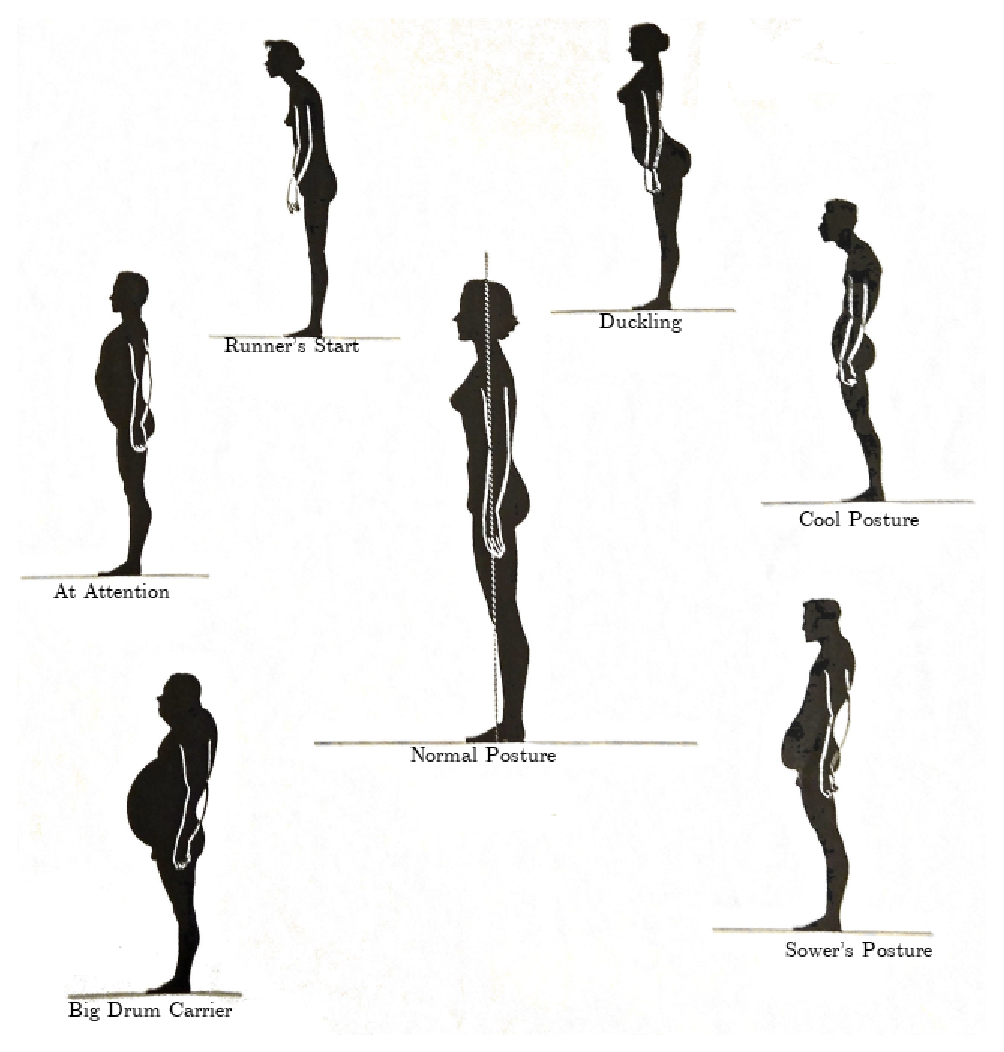
\includegraphics[width=1\linewidth]{Wrong_Postures}
\column{.3\textwidth} % Left column and width
Our posture is influenced by our \structure{habits and patterns}. It is the manifestation of our feelings.
\end{columns}
\end{frame}
%------------------------------------------------
%------------------------------------------------

\begin{frame}
\frametitle{Permanent stress in the brain}
\begin{columns}[c] % The "c" option specifies centered vertical alignment while the "t" option is used for top vertical alignment
\column{.7\textwidth} % Left column and width
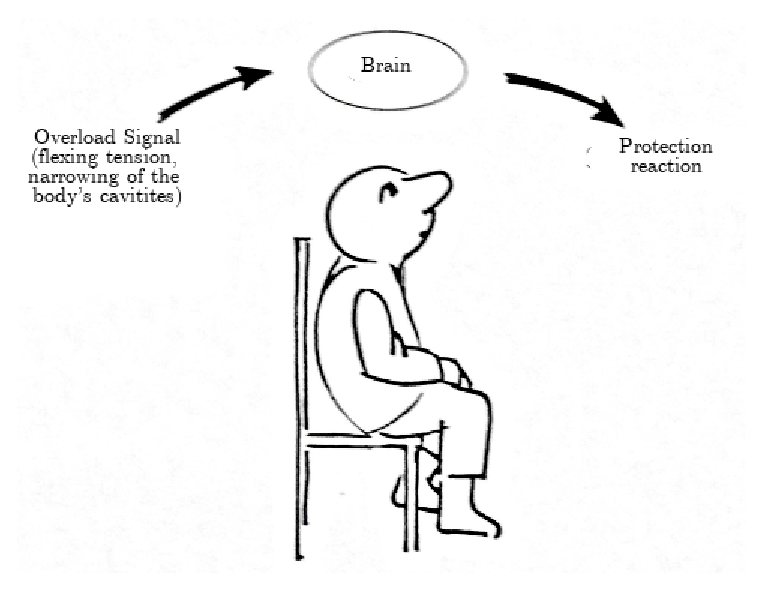
\includegraphics[width=1\linewidth]{Sitting_guy}
\begin{block}{-- Winston Churchill}
``\textit{You must offer something good to the body so that the soul wants to live in it. }''
\end{block}
\column{.3\textwidth} % Left column and width
The strain from a malposition needs to be overcome, else it constantly sends \structure{over--taxation signals} to the brain, which in turn cause \structure{protective measures} of the body which hold our body back from correcting our posture. That means \structure{permanent stress}.
\end{columns}
\end{frame}
%------------------------------------------------
\begin{frame}
\frametitle{Posture, equilibrium and feelings}

\begin{block}{-- Ch. Selver and Ch. Brooks}
``\textit{When we are standing relaxedly and are in equilibrium, we are investing exactly the amount of energy to counteract gravity and to truly perceive our whole organism. We can forgo the use of our eyes and solely rely on our feelings when we truly want to orient ourselves.\\
We gradually get aware that the smallest shift in body weight cause different sensations of effort or relief in our musculature or breath. When we close in on the equilibrium, a feeling of weightlessness, freedom, peace and happiness which isn't comparable to any other experience. We discover that we are in a constant flow state, nothing is static.}''
\end{block}


\begin{block}{-- Eric Franklin}
``\textit{The intellectual experience changes little, the experience on the level of the body brings the tranformation.}''
\end{block}
\end{frame}
%------------------------------------------------